%!TEX TS-program = pdflatexmk

% Copyright (c) 2018 - 2022, Martin Scheidt (ISC license)
% Permission to use, copy, modify, and/or distribute this file for any purpose with or without fee is hereby granted, provided that the above copyright notice and this permission notice appear in all copies.

\documentclass[border=2]{standalone}

\usepackage[dev]{tikz-trackschematic}

\begin{document}
  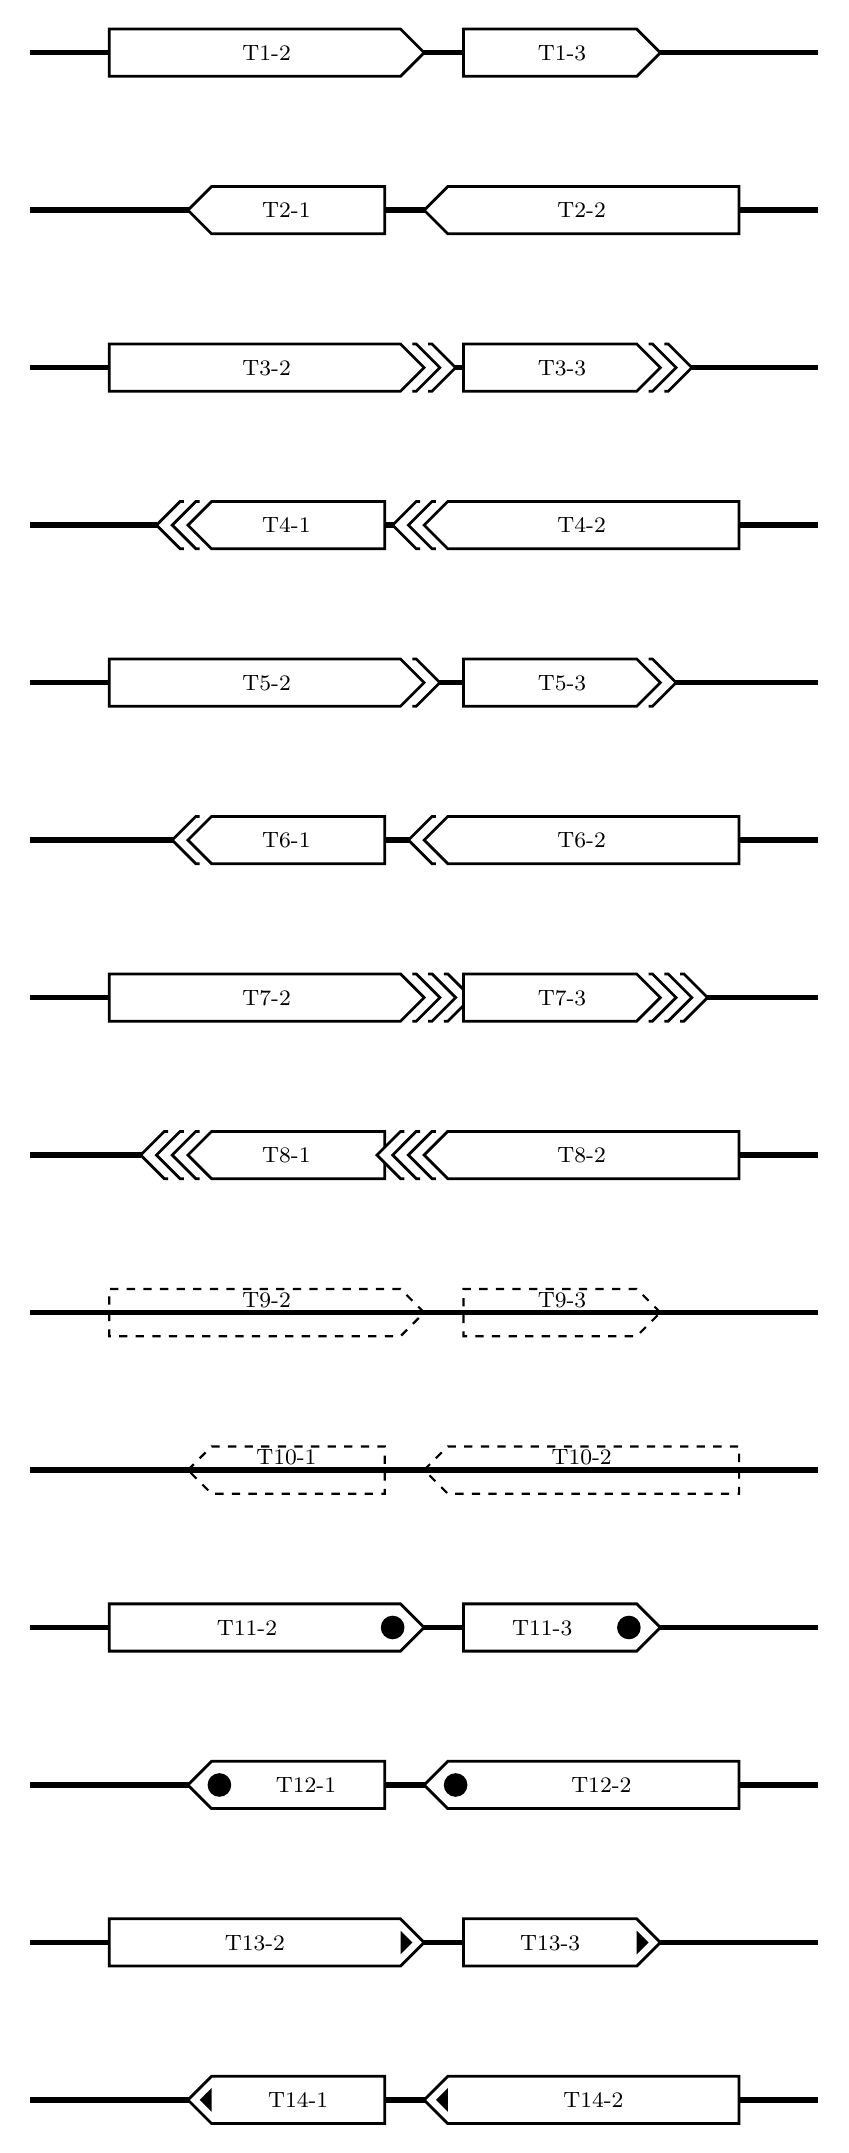
\begin{tikzpicture}
  
    \foreach \i in {1,2,...,14}{% base coordinate
      \coordinate (A\i) at ($(-1,0) + 2*(0,-\i)$);
      \coordinate (B\i) at ($( 9,0) + 2*(0,-\i)$);
    }

    \foreach \i in {1,2,...,14}{% draw main tracks on base coordinate
      \maintrack (A\i) --   (B\i);
    }

    \foreach \i in {1,2,...,14}{% coordinates for testing symbols
      \coordinate (T\i-1) at ($(1,0) + 2*(0,-\i)$);
      \coordinate (T\i-2) at ($(4,0) + 2*(0,-\i)$);
      \coordinate (T\i-3) at ($(7,0) + 2*(0,-\i)$);
    }

    \train[forward]               at (T1-2) label (T1-2);
    \train[forward ,length=2.5cm] at (T1-3) label (T1-3);
    \train[backward,length=2.5cm] at (T2-1) label (T2-1);
    \train[backward]              at (T2-2) label (T2-2);

    \train[run=normal,forward]               at (T3-2) label (T3-2);
    \train[run=normal,forward ,length=2.5cm] at (T3-3) label (T3-3);
    \train[run=normal,backward,length=2.5cm] at (T4-1) label (T4-1);
    \train[run=normal,backward]              at (T4-2) label (T4-2);

    \train[run=slow,forward]               at (T5-2) label (T5-2);
    \train[run=slow,forward ,length=2.5cm] at (T5-3) label (T5-3);
    \train[run=slow,backward,length=2.5cm] at (T6-1) label (T6-1);
    \train[run=slow,backward]              at (T6-2) label (T6-2);

    \train[run=fast,forward]               at (T7-2) label (T7-2);
    \train[run=fast,forward ,length=2.5cm] at (T7-3) label (T7-3);
    \train[run=fast,backward,length=2.5cm] at (T8-1) label (T8-1);
    \train[run=fast,backward]              at (T8-2) label (T8-2);

    \train[ghost,forward]               at (T9-2) label (T9-2);
    \train[ghost,forward ,length=2.5cm] at (T9-3) label (T9-3);
    \train[ghost,backward,length=2.5cm] at (T10-1) label (T10-1);
    \train[ghost,backward]              at (T10-2) label (T10-2);

    \train[operation=manual,forward]               at (T11-2) label (T11-2);
    \train[operation=manual,forward ,length=2.5cm] at (T11-3) label (T11-3);
    \train[operation=manual,backward,length=2.5cm] at (T12-1) label (T12-1);
    \train[operation=manual,backward]              at (T12-2) label (T12-2);

    \train[operation=automatic,forward]               at (T13-2) label (T13-2);
    \train[operation=automatic,forward ,length=2.5cm] at (T13-3) label (T13-3);
    \train[operation=automatic,backward,length=2.5cm] at (T14-1) label (T14-1);
    \train[operation=automatic,backward]              at (T14-2) label (T14-2);

  \end{tikzpicture}
\end{document}